\section{SOA}

La información contenida en la actual sección es tomada del libro \textit{Soa principles of service design} \cite{soa_principles}

\subsection{Primeros conceptos}

Los conceptos base del diseño de software deben ser expuestos para tener una mayor claridad en los temas siguientes. A continuación se expresan los conceptos base:

\begin{itemize}
  \item \textbf{Características de diseño}: Son aquellos atributos que cumple un diseño y que pueden ser medidos.
  \item \textbf{Principio de diseño}: Es una guía o regla para solucionar un problema de acuerdo a las prácticas aceptadas por la comunidad de ingeniería de software.
  \item \textbf{Paradigma de diseño}: Es el compendio de principios de diseño que tienen un enfoque global común.
  \item \textbf{Patrones de diseño}: Son formas de resolver un problema de diseño que es repetitivo. Viene dado por 3 restricciones presentadas en el diseño de software:
  \begin{itemize}
    \item Restricciones impuestas por la tecnología existente
    \item Restricciones impuestas por las tecnologías usadas por sistemas transversales
    \item Restricciones de prioridades de proyectos
  \end{itemize}
  El patrón de diseño describe el problema y da la solución a modo de plantilla.
  \item \textbf{Lenguajes de patrones de diseño}: Es la configuración ordenada de patrones en un diseño lógico. La comunicación entre cada patrón se hace a través de dicho lenguaje.
  \item \textbf{Estándares de diseño}: En orden de ir acorde a las metas, prioridades, recursos y ambiente de la organización en la que se haga el diseño lógico de la solución, un estándar de diseño define convenciones para cada elemento utilizado en el diseño de acuerdo a las características de diseño definidas.
  \item \textbf{Buenas prácticas}: Es una técnica o acercamiento para resolver o prevenir problemas presentados en el desarrollo del diseño lógico de la solución de software. pg 34
\end{itemize}

\begin{figure}[!htb]
  \begin{center}
    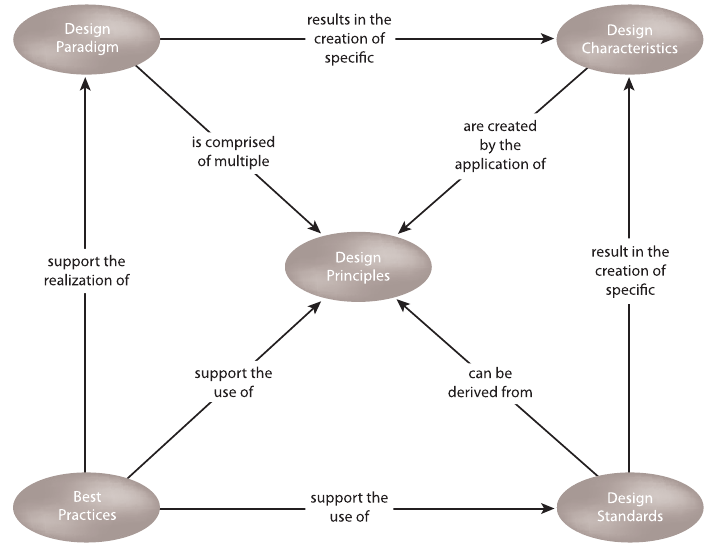
\includegraphics[width=11cm]{./imagenes/1.png}
    \caption{Acercamiento a cómo se desarrollan los principios de diseño con los demás conceptos nombrados.}
    \label{fig:uno}
    \textbf{Fuente:}  \cite{soa_principles}
  \end{center}
\end{figure}

La figura \ref{fig:uno} presenta un acercamiento a cómo se desarrollan los principios de diseño con los demás conceptos nombrados.

\begin{figure}[!htb]
  \begin{center}
    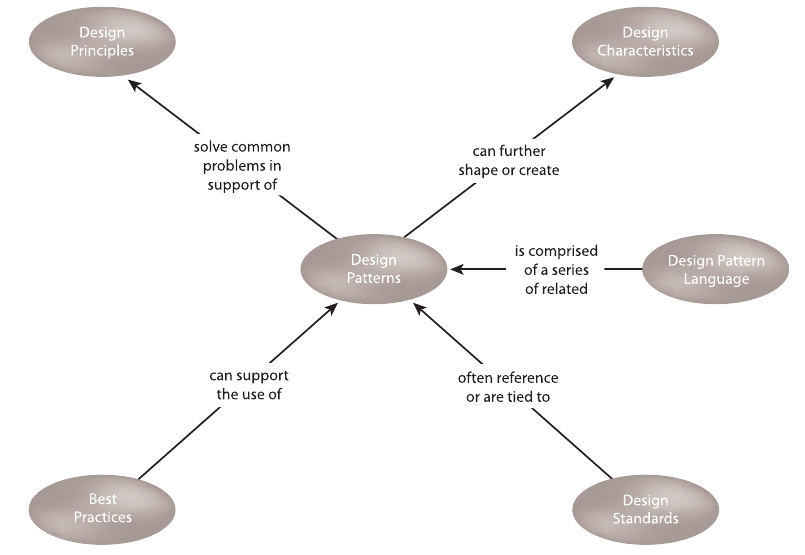
\includegraphics[width=11cm]{./imagenes/2.png}
    \caption{Como extiende o soporta un patrón de diseño el diseño lógico de la solución de software.}
    \label{fig:dos}
    \textbf{Fuente:}  \cite{soa_principles}
  \end{center}
\end{figure}

La figura \ref{fig:dos} presenta cómo extiende o soporta un patrón de diseño el diseño lógico de la solución de software.

\begin{figure}[!htb]
  \begin{center}
    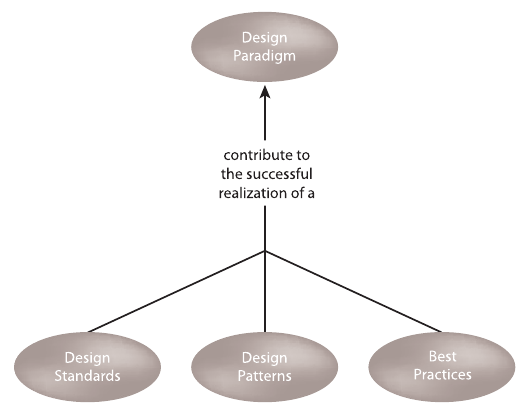
\includegraphics[width=11cm]{./imagenes/3.png}
    \caption{Componentes que hacen que el diseño lógico de la solución sea acorde al paradigma escogido.}
    \label{fig:tres}
    \textbf{Fuente:}  \cite{soa_principles}
  \end{center}
\end{figure}

La figura \ref{fig:tres} presenta los componentes que hacen que el diseño lógico de la solución sea acorde al paradigma escogido.

\subsection{Computación orientada a servicios}

La computación orientada a servicios nace de la necesidad de desarrollar software integrado con otros construidos con diferentes arquitecturas y, por ende, diversas tecnologías. Este tipo de computación tiene como finalidad la construcción de inventarios de servicios. La computación orientada a servicios está compuesta por la interacción de la orientación a servicios (paradigma de diseño) y la arquitectura orientada a servicios, formando patrones de diseño propios y estándares en cumplimiento de las características de diseño propias de la computación orientada a servicios. 

Algunos de los conceptos clave llevados en la computación orientada a servicios son:

\begin{itemize}
  \item Arquitectura Orientada a Servicios (SOA - Service Oriented Architecture): Comprende el compendio de tecnologías, APIs, infraestructura y repositorios enmarcados en el paradigma orientado a servicios y cuyo objetivo principal es el de trabajar sobre el "servicio" como el elemento más importante.
  \item Orientación a servicios: Es el paradigma manejado en la computación orientada a servicios en donde se acepta como unidad mínima y más importante el "servicio".
  \item Servicio: Es un software independiente físicamente el cual tiene asignado un contexto de funcionalidades y que puede ser utilizado por otros servicios por medio del contrato del servicio (descripción del servicio en cuanto a funcionalidades, entradas requeridas y salidas). De acuerdo a su nivel de reúso, los servicios se dividen en 3 tipos y son:
  \begin{itemize}
    \item Servicios entidad: Modela los servicios que se deben ofrecer respecto de las entidades del negocio (ej. empleados y clientes). Tienen un nivel de reúso alto y están centrados en el negocio.
    \item Servicios tarea: Modela los servicios que deben cumplir tareas específicas del negocio (ej. generación de cortes de final de año). Tienen un nivel de reúso bajo. Estos servicios trabajan directamente con 1 o varios servicios entidad. Estos servicios están centrados en el negocio.
    \item Servicios utilidad: Modela servicios que no están centrados en el negocio. Son los servicios con mayor reúso.
  \end{itemize}
\end{itemize}

\begin{figure}[!htb]
  \begin{center}
    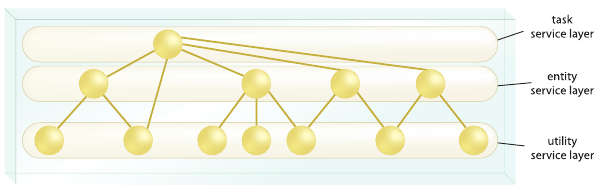
\includegraphics[width=11cm]{./imagenes/5.png}
    \caption{diferenciación entre tipos de servicio da lugar a la estructura en capas}
    \label{fig:cinco}
    \textbf{Fuente:}  \cite{soa_principles}
  \end{center}
\end{figure}

La diferenciación entre tipos de servicio da lugar a la estructura en capas mostrada en la figura \ref{fig:cinco}

\begin{itemize}
  \item Composición de servicios: Es la agregación de servicios de manera ordenada.
  \item Inventario de servicios: Es la agrupación de varios servicios según un criterio definido por la organización. Cada inventario de servicios tiene su propio estándar de diseño e, inclusive, su propia configuración arquitectónica. El desarrollo de los inventarios de servicio es hecho a modo top-down, con la construcción de blueprints, también llamados modelo de servicios de negocio o modelos de inventario de servicios.
\end{itemize}

\begin{figure}[!htb]
  \begin{center}
    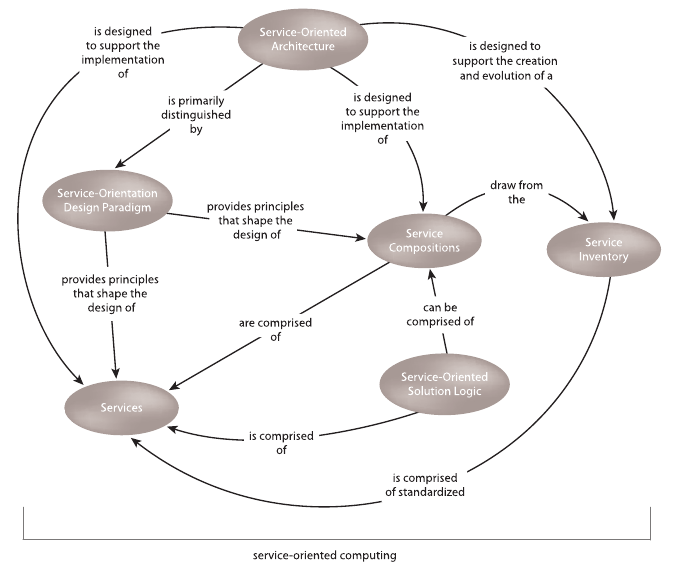
\includegraphics[width=11cm]{./imagenes/4.png}
    \caption{Interacción de los conceptos clave en la computación orientada a servicios}
    \label{fig:cuatro}
    \textbf{Fuente:}  \cite{soa_principles}
  \end{center}
\end{figure}

\subsection{Proceso de Análisis y diseño orientados a servicios}

En la etapa de análisis y diseño, el arquitecto de software se reúne con un analista de negocio, el cual diseñará unos servicios candidatos que después se convertirán en los servicios incluidos en los blueprints. Luego de tener los planos, el arquitecto escoge un subconjunto de dichos candidatos a servicios para ser implementados físicamente, dotándolos de algún método para realizar la composición de servicios. En la \ref{fig:seis} se muestra el proceso de análisis y diseño orientado a servicios.

\begin{figure}[!htb]
  \begin{center}
    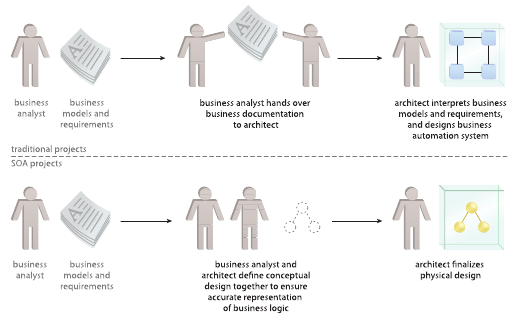
\includegraphics[width=11cm]{./imagenes/6.png}
    \caption{proceso de análisis y diseño orientado a servicios}
    \label{fig:seis}
    \textbf{Fuente:}  \cite{soa_principles}
  \end{center}
\end{figure}

\subsection{Metas y beneficios de la computación orientada a servicios }

Las metas y los beneficios que trae la implementación de la computación orientada a servicios en una organización son:

\begin{itemize}
  \item \textbf{Incremento de la interoperabilidad intrínseca}: Es una meta de la computación orientada a servicios ya que la composición de servicios requiere que, sin necesidad de integrar un servicio con el otro, estos puedan intercambiar información para desarrollar la funcionalidad a la que han sido inscritos. Aplicando principios de diseño orientados a servicios, así como también estándares de diseño orientados a servicios, se logra el incremento de la interoperabilidad intrínseca.
  \item \textbf{Federación incrementada}: Un entorno de TI federado es aquel en el cual los recursos y aplicaciones se manejan y gobiernan con autonomía y por sí mismos. En el ámbito de la orientación a servicios, cada servicio puede tener su propia implementación independiente y aun así comunicarse. Esto se logra por medio de una especial atención a los estándares de diseño.
  \item \textbf{Incremento de opciones en la escogencia de proveedores de servicios}: Como la federación en la computación orientada a servicios es una meta, la escogencia de proveedores de servicios diferentes es un beneficio ya que la composición de servicios puede ser lograda sin importar que proveedor provea de un servicio específico.
  \item \textbf{Incremento de la alineación entre el negocio y las tecnologías}: Ya que en el proceso de diseño actúan tanto el analista de negocio como el arquitecto de software, la alineación entre negocio y tecnologías es incrementada. La reconfiguración en la composición de servicios, además, provee alineación extra al poder cambiar el proceso de negocio y la composición de los servicios al mismo tiempo.
  \item \textbf{ROI}: Al hacerse inventarios de servicios y, además, ser los servicios reutilizables a lo largo del tiempo y compuestos de diferente forma gracias a la composición de servicios, se da una relación costo/beneficio más baja que con otros paradigmas usados.
  \item \textbf{Agilidad organizacional incrementada}: Debido a la orientación a servicios, se hace una composición rápida de los servicios que se tengan y se crean los que se necesiten para agilizar el proceso del departamento de TI y así agilizar los procesos subyacentes.
  \item \textbf{Reducción de cargas al departamento TI}: Debido a la agilidad organizacional cuando es aplicada la orientación a servicios, son reducidos costos operacionales (tiempo u otros recursos) y el departamento de TI adquiere un papel activo en el sector estratégico.
\end{itemize}
